\documentclass{article} % For LaTeX2e
\usepackage{nips14submit_e,times}
\usepackage{hyperref}
\usepackage{url}
%\documentstyle[nips14submit_09,times,art10]{article} % For LaTeX 2.09
\usepackage{graphicx,subcaption}              % to include figures
\usepackage{epstopdf}
\usepackage{amsmath}               % great math stuff
\usepackage{amsfonts}              % for blackboard bold, etc
\usepackage{amsthm}                % better theorem environments

\usepackage{notoccite}
\usepackage[numbers,sort&compress]{natbib}
\usepackage{array}
\title{Multiple Sclerosis Lesion Segmentation in MRI Images }

\author{
Gautham Vasan \\
Department of Computing Science\\
University of Alberta\\
%Edmonton, T6E2H2 \\
\texttt{vasan@ualberta.ca} \\
\And
Jared Rewerts \\
Department of Computer Engineering \\
University of Alberta \\
%Edmonton, T6E2H2 \\
\texttt{rewerts@ualberta.ca} \\
\And
Megha Panda \\
Department of Computing Science\\
University of Alberta \\
%Edmonton, T6E2H2 \\
\texttt{meghaanu@ualberta.ca} \\
\texttt{email} \\
\And
Parisa Mohebbi \\
Department of Computing Science \\
University of Alberta \\
%Edmonton, T6E2H2 \\
\texttt{mohebbi@ualberta.ca} \\
\And
Reza Sobhannejad \\
Department of Computing Science \\
University of Alberta \\
%Edmonton, T6E2H2 \\
\texttt{sobhanne@ualberta.ca} \\
\And
Sina Jalali  \\
Department of Computing Science \\
University of Alberta \\
%Edmonton, T6E2H2 \\
\texttt{jalali1@ualberta.ca} \\
}

% The \author macro works with any number of authors. There are two commands
% used to separate the names and addresses of multiple authors: \And and \AND.
%
% Using \And between authors leaves it to \LaTeX{} to determine where to break
% the lines. Using \AND forces a linebreak at that point. So, if \LaTeX{}
% puts 3 of 4 authors names on the first line, and the last on the second
% line, try using \AND instead of \And before the third author name.

\newcommand{\fix}{\marginpar{FIX}}
\newcommand{\new}{\marginpar{NEW}}

\nipsfinalcopy % Uncomment for camera-ready version

\begin{document}


\maketitle
% Abstract
\begin{abstract}
Magnetic Resonance Imaging (MRI) is commonly used to detect Multiple Sclerosis Lesions in the Central Nervous System. As the lesions are anatomically  variable, accurate segmentation of MS lesions is challenging. Since manual segmentation requires domain knowledge and is usually expensive and time consuming, we aim to automatically segment lesions. Our focus is on comparing classification techniques using a wide range of features for Multiple Sclerosis lesion segmentation in order to find the most successful techniques. We also attempt to combine some techniques to improve detection success. Our results indicate that Markov Random Fields with Random Forest provides the best result and that there are other options useful in segmenting lesions. Interestingly, Random Forest is better choice in terms of computational complexity than other algorithms, especially when compared to SVM. This makes it the most practical in terms of both accuracy and speed. 
\end{abstract}

%---------------------------------------- Introduction-------------------------------------------%
\section{Introduction}
%What is MS? Why it is an interesting problem? Problem definition and motivation. What are the challenges?
Multiple Sclerosis (MS) is a debilitating disease that affects the brain and spinal cord.  MS is an autoimmune disease where the immune system attacks parts of the body, in this case, the protective covering of nerve fibers. If occurrences are bad enough, the nerves can build up scar tissue, which impedes nerve conduction. This scar tissue is what we refer to as lesions. One of the most shocking aspects of Multiple Sclerosis is that it primarily affects individuals between the ages of 15 and 40. Women are also twice as likely to be affected by MS. Early detection is key to managing symptoms and controlling the disease outcomes. Affected individuals can use exercise, cool temperatures and a balanced diet to mitigate the symptoms.

Detection of MS lesions is done using scans of patient brains. Medical professionals analyze these scans, looking for signs of MS. These manual segmentation techniques are usually expensive, time consuming and require domain specific knowledge. As there is no consensus among different experts, we do not have a gold standard for validation of the classification techniques. Automatic segmentation techniques are being increasingly used in a hope to alleviate these issues. 

One of the main challenges of automatic segmentation is the low lesion volume in patient brain matter. Typically, only a small percentage of the patients brain has lesions, which makes detection highly challenging. The ratio of positive to negative data samples is considerably low compared to many other segmentation problem spaces which makes the data biased. Furthermore, since most patients have very little scar tissue, over classification is one of the issues with automated segmentation. Ideally, if a healthy brain is scanned and processed, we would show no lesions. In practice, this can be an arduous task.


\subsection{Related Work}
Segmentation of Lesions in MRI images is an active area of research. The 3 main objectives are: 
\begin{enumerate}
  \item Extracting features that can differentiate healthy tissues from scar tissues, 
  \item Selecting the most relevant features that help achieve the task, and
  \item Improving the performance of the classification.
\end{enumerate} 

\subsubsection{Review of Segmentation Methods}
In MS lesion segmentation, the typical features are the intensity of each voxel in different image modalities. Additionally, some methods like  \cite{commowick2009continuous}, combined K-Nearest Neighbours (k-NN) based on intensities with a template-driven segmentation method to reduce false positives. The method presented in \cite{zijdenbos2002automatic} used the probability of a voxel belonging to tissue class with help of an atlas. Intensity of the six neighbor voxels can be added to feature vector of a point which has been used with an Artifical Neural Networks in \cite{younis2007ms}. In \cite{kroon2008multiple}, they extracted up to 255 features derived by applying different filters on every image. Later, with the help of Principal Component Analysis (PCA), data is transformed to new orthogonal coordinates so that the first column covers the greatest variance between data.  Hence, a simple thresholding on the first component of PCA can classify lesions. In \cite{geremia2011spatial}, Random Decision Forest (RDF) is used with local (e.g., intensity features) and context-rich (discussed later) features. RDF has the advantage of automatically selecting the best features over other methods.

\subsubsection{ Exploring Combinations }
Lots of methods have been employed for lesion segmentation as mentioned before but no valid comparison is done to measure performance of different classifiers using different features. In this project we aim to compare various algorithm's efficiencies on the same data and feature sets to explore their properties in  lesion segmentation. We use Support Vector Machine (SVM), Neural Networks, K-Nearest Neighbors, Random Forest, Markov Random Field, and Logistic Regression as classifiers. For features, we use Haar-Like, image filters, LM filters, entropy, gaussian based, and atlas. In a broad sense, we tried to extract all possible features to see how the well-known classifiers operate based on them.

%------------------------------------------- Features ----------------------------------------------%
\section{Feature Detection}
%What is feature extraction? Why is it important? Reasons for using the particular features
Image analysis aims at reducing information to a subset that is relevant to the task in hand. Information reduction often happens gradually with information being reduced until the desired result is extracted from the data. \cite{toennies2012guide} The first level of reduction computes local features that are assumed to pertain to objects of interest. We use 4 different classes of features here in order to segment the MRI images. The features we use for the given task were selected based on the literature survey for MS Lesion segmentation described in the Related Work section. The general characteristics and reasons for why the particular class of features work is described below.  

\subsection{Context (Haar-Like Features)}
In the detection phase of the Viola-Jones object detection framework \cite{Viola-Jones}, a window of the target size is moved over the input image, and for each subsection of the image the Haar-like feature is calculated. This difference is then compared to a learned threshold that separates non-objects from objects. Because such a Haar-like feature is only a weak learner or classifier (its detection quality is slightly better than random guessing) a large number of Haar-like features are necessary to describe an object with sufficient accuracy. Context-rich features exhibit high variability. This variability combined with their ability to highlight regions which differ from their neighborhood explains why they were chosen. Together with local features (voxel intensities), context-rich features learn a multichannel appearance model conditioned by tissue spatial priors.\cite{geremia2011spatial}

\begin{figure}[h]
\centering
\begin{subfigure}[b]{.4\linewidth}
\centering
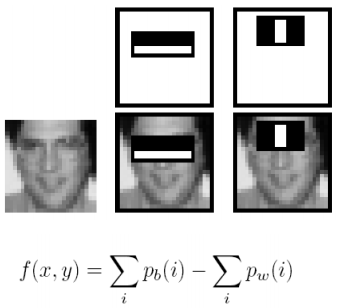
\includegraphics[scale=0.3]{haar}
\caption{ Calculation of Haar-like feature}
%\label{fig:subim1}
\end{subfigure}
\begin{subfigure}[b]{.4\linewidth}
\centering
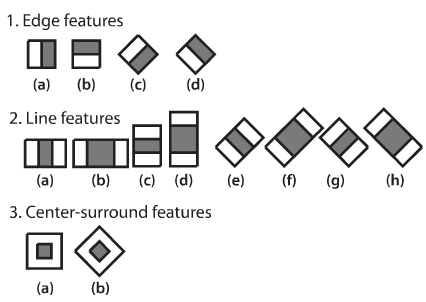
\includegraphics[scale=0.3]{HaarFeatures}
\caption{Different types of Haar-like Features}
%\label{fig:subim2}
\end{subfigure}
\caption{Haar-Like Features}
\end{figure}

\subsection{Image Filters}
Filtering is a technique used for modifying or enhancing an image. It can be used to emphasize certain features or remove other features in an image. In image processing filters are mainly used to suppress either the high frequencies in the image, i.e. smoothing the image, or the low frequencies, i.e. enhancing or detecting edges in the image. We extract the features through Linear filtering of the MRI image using convolution. 

\subsubsection{Leung-Malik (LM) Filter Bank}
We use the filter bank provided by the Visual Geometry Group at the University of Oxford to obtain a set of features. The LM set is a multi scale, multi orientation filter bank with 48 filters. It consists of first and second derivatives of Gaussians at 6 orientations and 3 scales making a total of 36; 8 Laplacian of Gaussian (LOG) filters; and 4 Gaussians. The filters occur at the basic scales $\sigma$ = {$\sqrt{2}$,2,2$\sqrt{2}$,4}. The Gaussians occur at the four basic scales while the 8 LOG filters occur at $\sigma$ and 3$\sigma$. The algorithm proposed by Leung and Malik \cite{LMfilters} demonstrated excellent
results for recognizing 3D textures from a single image under any lighting and viewing geometry. Since different MRI scanners produce different quality of images, the LM filters should be able to recognize different textures, i.e., lesions in the brain.
\begin{figure}[h]
\centering
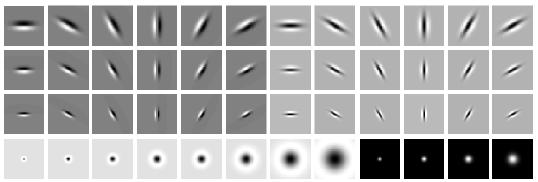
\includegraphics[scale=0.3]{lmfilters.jpg}
\caption{LM filters - Edge, bar and spot filters at multiple scales and orientations.}
\label{fig:LM filters}
\end{figure}

\subsection{Entropy \& Gaussian based Features}

Entropy measures the randomness of each of the pixel.It accounts for all the randomness for a patch, that can be varied. Entropy of each of the pixel depends on 5*5 patch surrounding neighbour point. One of the main reasons to choose entropy as a feature is, the pixel not only accounts for its own value, but also considers the surroundings, which helps the classifier to train better.
Guassian features are nothing but,a filter  that filters the image with a 2-D Gaussian smoothing kernel with standard deviation of 0.5.The sigma can vary, we chose it to be 2 for our experiment.

\begin{figure}[h]
\centering
\begin{subfigure}[b]{.4\linewidth}
\centering
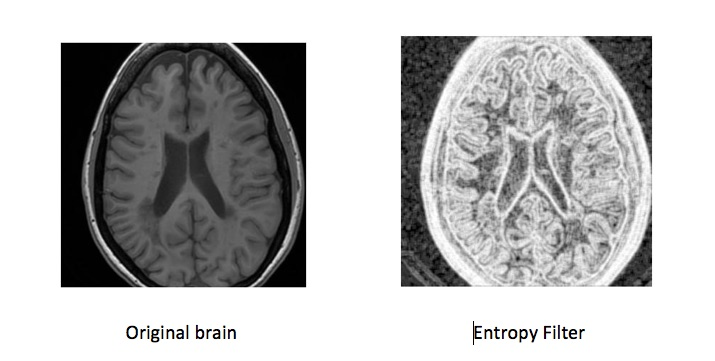
\includegraphics[scale=0.2]{entropy.jpg}
\caption{ Application of Entropy filter.}
%\label{fig:subim1}
\end{subfigure}
\begin{subfigure}[b]{.4\linewidth}
\centering
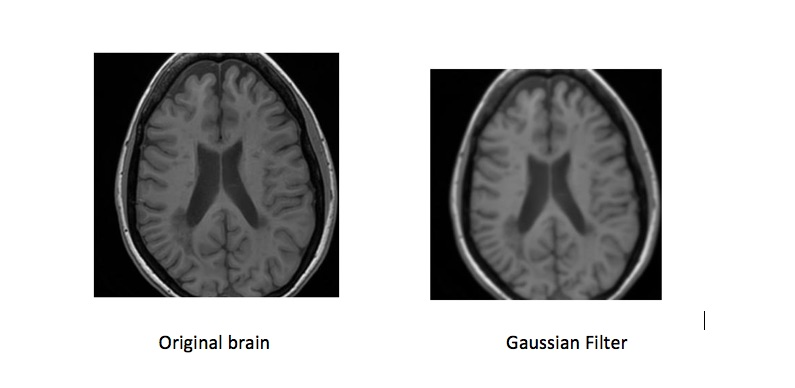
\includegraphics[scale=0.2]{gauss.jpg}
\caption{Application of Gaussian filter.}
%\label{fig:subim2}
\end{subfigure}
\caption{Entropy \& Gaussian based Features}
\end{figure}


\subsection{Atlas Features}

To pool the result across different subjects, we need to register the brain on each other or to register a set of brains to a common space/template. There are 2 kinds of registration; linear and non linear. FLIRT is an example of a software that performs linear registration, meaning that it will translate, rotate, zoom and shear one image to match it with another. Sometimes the differences between subjects are such that the linear transform is not sufficient to achieve good registration. The local deformations permitted by a non-linear method may then do a better job. 
We use FNIRT (non-linear) \cite{fnirt} of fsl\cite{fsl1}\cite{fsl2}\cite{fsl3} to achieve this. As most of the observed lesion are expected to be in the white matter, we want the Brain to be trained only on white matter for better accuracy. We use this as a feature. FAST \cite{fast} (FMRIB's Automated Segmentation Tool) segments a 3D image of the brain into different tissue types (Grey Matter, White Matter, CSF, etc.), whilst also correcting for spatial intensity variations (also known as bias field or RF inhomogeneities). The underlying method is based on a hidden Markov random field model and an associated Expectation-Maximization algorithm. The whole process is fully automated and can also produce a bias field-corrected input image and a probabilistic and/or partial volume tissue segmentation. It is robust and reliable, compared to most finite mixture model-based methods, which are sensitive to noise. 
\begin{figure}[h]
\centering
\begin{subfigure}[b]{.3\linewidth}
\centering
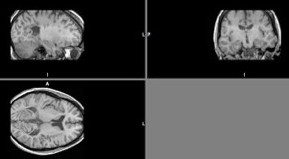
\includegraphics[scale=0.25]{atlas1.jpg}
\caption{ Original Brain.}
%\label{fig:subim1}
\end{subfigure}
\begin{subfigure}[b]{.3\linewidth}
\centering
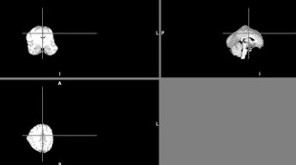
\includegraphics[scale=0.25]{Atlas2.jpg}
\caption{Non Linear Registration}
%\label{fig:subim2}
\end{subfigure}
\begin{subfigure}[b]{.3\linewidth}
\centering
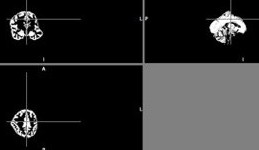
\includegraphics[scale=0.25]{atlas3.jpg}
\caption{ Segemented Brain.}
%\label{fig:subim3}
\end{subfigure}
\caption{Atlas Features}
\end{figure}


%------------------------------------------------ Classifiers ------------------------------------------%
\section{Classifiers}
%Reasons for using each classification method. Brief description about them. No need for images here I guess.

The general characteristics of each classifier used and the reasons for choosing them for the given task is given below. 
\subsection{Support Vector Machines (SVM)} 
SVMs try to split the positive and negative data using a hyper-plane which works very well on complex tasks when implemented with kernels. The model is both powerful and unlikely to over-fit. But it is sensitive to the ratio of positive and negative data (pos/neg) as it weights them equally. In our case, we need a model to learn lots of negative data, healthy brain patches, and a few positive data samples. Hence, we sample the training data such that it is not unbalanced, i.e., never more than a ratio of 2 to 1.

\subsection{ Neural Networks} 
The most important property of neural networks is the ability to identify a good estimation even for complex functions. Basically in Neural Networks we have a few layers. The first layer is our features (input) and the last layers is related to the labels (output). We also have a few hidden layers between these two. Considering this structure we can make almost all functions, even the most complex ones. That’s the reason for choosing this method. In this project we tried Neural Networks with 2 to 3 hidden layers.

\subsection{k-Nearest Neighbours} 
Nearest Neighbours approach decides on the label of a certain data-point by counting votes of its k closest points. The model is completely dependent on the distance measure used to find close points. It is easy to implement this model and does not require training. To make a decision on each voxel we take the majority of votes from nearest points in the dataset. 

\subsection{Random Forests (RF)} 
The model is based on taking into account the votes of a set of decision trees on each voxel. One of the best properties of RFs is that they are less sensitive to imbalanced ratio of positive and negative data compared to other models. Also, it provides the best features which split the classes better and scores the features based on how helpful they are in classification. Furthermore, it is hard for RFs to overfit while they fit complex models as a result of using different trees to make the overall decision. We learn the random forest and create the trees by distributing points in their leafs and predict by merging votes of each tree to label the data.

\subsection{Markov Random Fields}
The basic principle of Markov Random Field is to treat the input image as a graph in which each voxel is a node and all the neighboring voxels are interconnected. In the case of foreground segmentation, two spatial nodes of foreground and background are added to the graph and edges between voxels. Each pair of nodes are assigned a weight equal to the probability that a given voxel belongs to either foreground or background. In graph theory, a cut is a partition of the vertices of a graph into two disjoint subsets. An st-cut is a graph cut comprising all directed edges from a node in a vertex set A to a node in its complement, $\overline{A}$, such that s $\epsilon$ A, t $\epsilon$ $\overline{A}$, and A is connected. The cost of a cut is simply defined as the sum of edge weights for the edges removed by the cut. The aim of this algorithm is to use a graph-cut to divide graph into two classes subject to the Min-Cut problem, i.e, to find the st-cut with minimal cost. The advantage of this method is that it considers the probabilities of its neighbours as a feature.

In this project, we trained a random forest (Claimed to be the best algorithm for lesion segmentation according to literature survey \cite{garcia2013review}) and used it to obtain initial probabilities of each voxel classified as a lesion. Subsequently, MRF is applied on the graph constructed using the weights,i.e., probabilities obtained from the classifier.

\subsection{Logistic Regression} 
The model fits a line to separate the classes of data. It is easily implemented and if it has sufficient features, is capable of doing well in our problem space. We learn the hyper-plane through our train data and classify test data based on the direction of the hyper-plain they fall into. A particular area of interest is how MRF improves logistic regression when used in sequence. Logistic Regression would also act as a simple measure of the effectiveness of the features used. The idea is that if logistic regression is able to perform nearly as well as Random Forest, the features are working well irrespective of the classifier used.  


%-----------------------------------Experiment Design -------------------------------------------------------%
\section{Experiment Design}
%Pipeline Diagram is required here

\subsection{Validation Measures}
For each pixel of the brain, our classifiers must label it as either lesion or healthy brain matter. Depending on the data set used, our ground truth source may be different. The MICCAI data set is provided by doctors and has also been cross referenced several times. The hope is that this increases the accuracy of the results. The MICCAI dataset represents real brain scans. Brain Web on the other hand uses a simulated brain scan and places lesions in the simulated scans.

When comparing our output to the ground truth, we come up with 4 possibilities for each region of the brain scan:
\begin{enumerate}
  \item True Positive - The ground truth and our detection agrees the region is a lesion.
  \item True Negative - The ground truth and our detection agrees the region is healthy.
  \item False Positive - Our detection finds a lesion in a brain region, but the ground truth disagrees.
  \item False Negative - The ground truth finds healthy brain, but our detection disagrees.
\end{enumerate} 
Taken together, these values can be used to analyze the performance of different classifiers. 
\subsubsection{Dice Score}
Dice is the primary metric we used to analyze algorithm performance. 

$$\frac{2*True Positive}{False Positive + False Negative + 2*True Positive}$$

One of the major benefits of Dice is that it heavily weights true positives. This makes it a very strict measure for a problem space like ours, where the amount of positive tissue is very low. As an example, consider scanning a brain that has a single tiny lesion. To get a perfect dice score, you must classify that lesion and only that lesion. Failing to classify that lesion will result in a score of 0. If you successfully classify the lesion, but also falsely classify surrounding tissue, the dice score will decrease rapidly. Since the healthy tissue heavily outweighs the lesions, it is easy to falsely classify a small amount of this healthy tissue as lesion.

There is one caveat to keep in mind when using Dice however. If we test against a healthy brain scan, Dice cannot be used to analyze our results. This is because there is no possibility of getting a true positive and so the result will always be 0.

\subsubsection{Accuracy}
Accuracy is good measure of how much brain matter we properly classify. Unlike Dice, accuracy weights true negatives evenly with true positives.

$$\frac{True Positive + True Negative}{False Positive + False Negative + True Positive + True Negative}$$

For our problem, accuracy usually isn't very useful. The reason for this is that true negatives are too common to be considered a reliable metric. For most brain scans, you could just classify the brain as healthy and the resulting accuracy would be good. We still use it though, as it can be useful when scanning healthy brains, which is where Dice fails.

\subsubsection{Sensitivity}

Sensitivity is similar to Dice in that it heavily weights true positives.

$$\frac{True Positive}{False Negative + True Positive}$$

Sensitivity affords no penalty to misclassifying healthy brain as lesion. This means a brain scan that is output as entirely lesion will do well on it. Despite this drawback, it can still be useful in situations that Dice is in.

\subsubsection{Detections}

As a simple evaluation measure, we count the number of properly classified lesions. A lesion is considered classified if we find even a single pixel of lesion within it. This makes it unreliable in terms of overall performance, but it is a valuable metric for basic testing of classifiers.

\subsection{Training and Test Data}
%BrainWeb and Miccai Challenge Data. Explain how sampling is done on data to train the classifier.
The quantitative analysis of the MRI images is done using data provided by two sources:
\begin{enumerate}
\item Brain Web - MS Lesion Brain Database, McGill University
\item MICCAI Challenge 2008 Dataset
\end{enumerate}

There exists no common ground truth or gold standard in most medical analysis tasks which results in an increasing need for validation of techniques. The Simulated Brain Database (SBD) acts as a stopgap solution to the validation problem. SBD is based on two anatomical models: (i) Normal brain and (ii) MS Lesion.  For both the models, full 3-dimensional data volumes have been simulated using three sequences (T1-, T2-, and proton-density- (PD-) weighted) and a variety of slice thicknesses, noise levels, and levels of intensity non-uniformity.  Unlike the vivo acquired data, here the ground truth is known which helps evaluating the various image analysis methods. 

The MICCAI challenge dataset is actual MRI image scans provided in 3 sequences - T1, T2 and Flair. The actual MRI image scans are obtained from Boston Children's Hospital (CHB) and University of North Carolina, Chapel Hill (UNC). The labels for the data are provided by two or more experts for each brain which results in a rough estimate for the presence of a lesion. We have 10 labeled brain volumes each from CHB and UNC as training data. Additionally, we have 18 unlabeled volumes from CHB and 10 unlabeled volumes from UNC as test data. The difficulty in using the MICCAI challenge data is that:
\begin{enumerate}
\item Less than 0.1\% of the brain volume is lesions
\item Different MRI Scanning devices result in different quality of images
\item No uniformly accepted Ground Truth or Gold Standard for validation
\end{enumerate}

Since the datasets are heavily biased, we sample the data from one volume on the brain and test on an entirely different volume of the brain. The sampling is done usually in a ratio 1:2 to 1:7 between positive and negative samples of data, where positive samples are considered to be lesions. For testing the classifier, the features are extracted for every pixel and tested on the entire volume of a brain.  

% --------------------------------------- Results ----------------------------------------------------%
\section{Results}
Lots of Images! Table with comparative results. Explanation for why we get these results. 

\begin{center}
\centering
\begin{tabular}{ | m{7em} | m{2cm}| m{2cm} | m{2cm} | m{2cm} | } 
\hline
\textbf{Classifier} & \textbf{Dice Score} & \textbf{Accuracy} & \textbf{Sensitivity} & \textbf{Detection}\\ 
\hline
SVM & 0 & 0 & 0 & 0  \\ 
\hline
Neural Networks & 0 & 0 & 0 & 0 \\ 
\hline
k-Nearest Neighbours & 0 & 0 & 0 & 0 \\ 
\hline
Random Forest & 0 & 0 & 0 & 0 \\ 
\hline
MRF with RF & 0 & 0 & 0 & 0 \\ 
\hline
Logistic Regression & 0 & 0 & 0 & 0 \\ 
\hline
\end{tabular}
\end{center}

\subsection{State of the art results}
The best results for segmenting MS lesions reported until now comes from random forest algorithm explained in \cite{geremia2011spatial}. Their proposed method contains of 30 separated decision trees with maximum depth of 20; each tree has a lower bound for information gain which stops it from further growing. They used two types of features, local features which are intensities and context-rich features which combine intensity of a single voxel with distant regions. This method is tested on MICCAI grand challenge 2008 and they got a dice score of $39.39 \pm 18.4$. This result comes from doing a 3-fold cross-validation, meaning model is trained on two different brains and tested on the third one and the procedure repeats for three times.\\
The important thing they revealed about MS lesion segmentation task is its need of having as more comprehensive training set as possible. They demonstrated that classifier with their selected features cannot detect lesions in locations which are not represented in training data.
\subsection{Discussion}
Detailed analysis of the results we get from different results

%-------------------------------------- Conclusion ------------------------------------------%
\section{Conclusion}
In this work we compared the performance of 6 different classifiers using 4 unique classes of features. We used the publicly available BrainWeb and MICCAI Challenge 2008 dataset for the problem of MS lesion segmentation in MRI images. MRF combined with RF gave the best dice score (0.00 \%) for the lesion segmentation task. Our results confirm the standard \cite{garcia2013review} that Random Forest typically provides the best results, but that MRF is able to enhance the dice score. Using MRF on RF improved the dice score by 0.00\%. Interestingly, Random Forest also tends to classify more quickly than other algorithms. Using RF we found that the following features were most useful for classification - [Should add the results here]. Using LDA for reducing the dimensionality could help speeding up the computational time required. Improving the sampling using Atlas features and using a wide range of context rich features could result in better performance of our classifier.


% ---------------------------------------- Acknowledgements ----------------------------------%
\section{Acknowledgements}


%------------------------------------------- References ----------------------------------------%
\section{References}

\bibliography{bibliography}
\bibliographystyle{plain}

\end{document}
